\documentclass{beamer}
\usepackage[english]{babel}
%\usepackage[utf8]{inputenc}
\usepackage[T1]{fontenc}
\usepackage{stmaryrd} %http://www.ctan.org/pkg/stmaryrd
\usepackage{amsmath} %http://www.ctan.org/pkg/amsmath
\usepackage{amssymb}
\usepackage{subfig}
\usepackage{hyperref}

\usetheme[usetitleprogressbar, numbering=fraction]{metropolis}

\graphicspath{{img/}}

\newcommand\bb{Benjamin Boisson}
\newcommand\gc{Guillaume Combette}
\newcommand\dl{Dimitri Lajou}
\newcommand\vl{Victor Lutfalla}
\newcommand\om{Octave Mariotti}
\newcommand\mr{Raphaël Monat}
\newcommand\me{Etienne Moutot} % He is not the only one author o/ Just that \em is already taken
\newcommand\js{Johanna Seif}
\newcommand\ps{Pijus Simonaitis}




\title{Blend'it}
\subtitle{Integrated project}
\author{\bb\\ \gc\\ \dl\\ \vl\\ \om\\ \mr\\ \me\\ \js\\ \ps\\}
\date{April 15th, 2016}

\begin{document}
\begin{frame}
\begin{figure}
  \begin{center}
    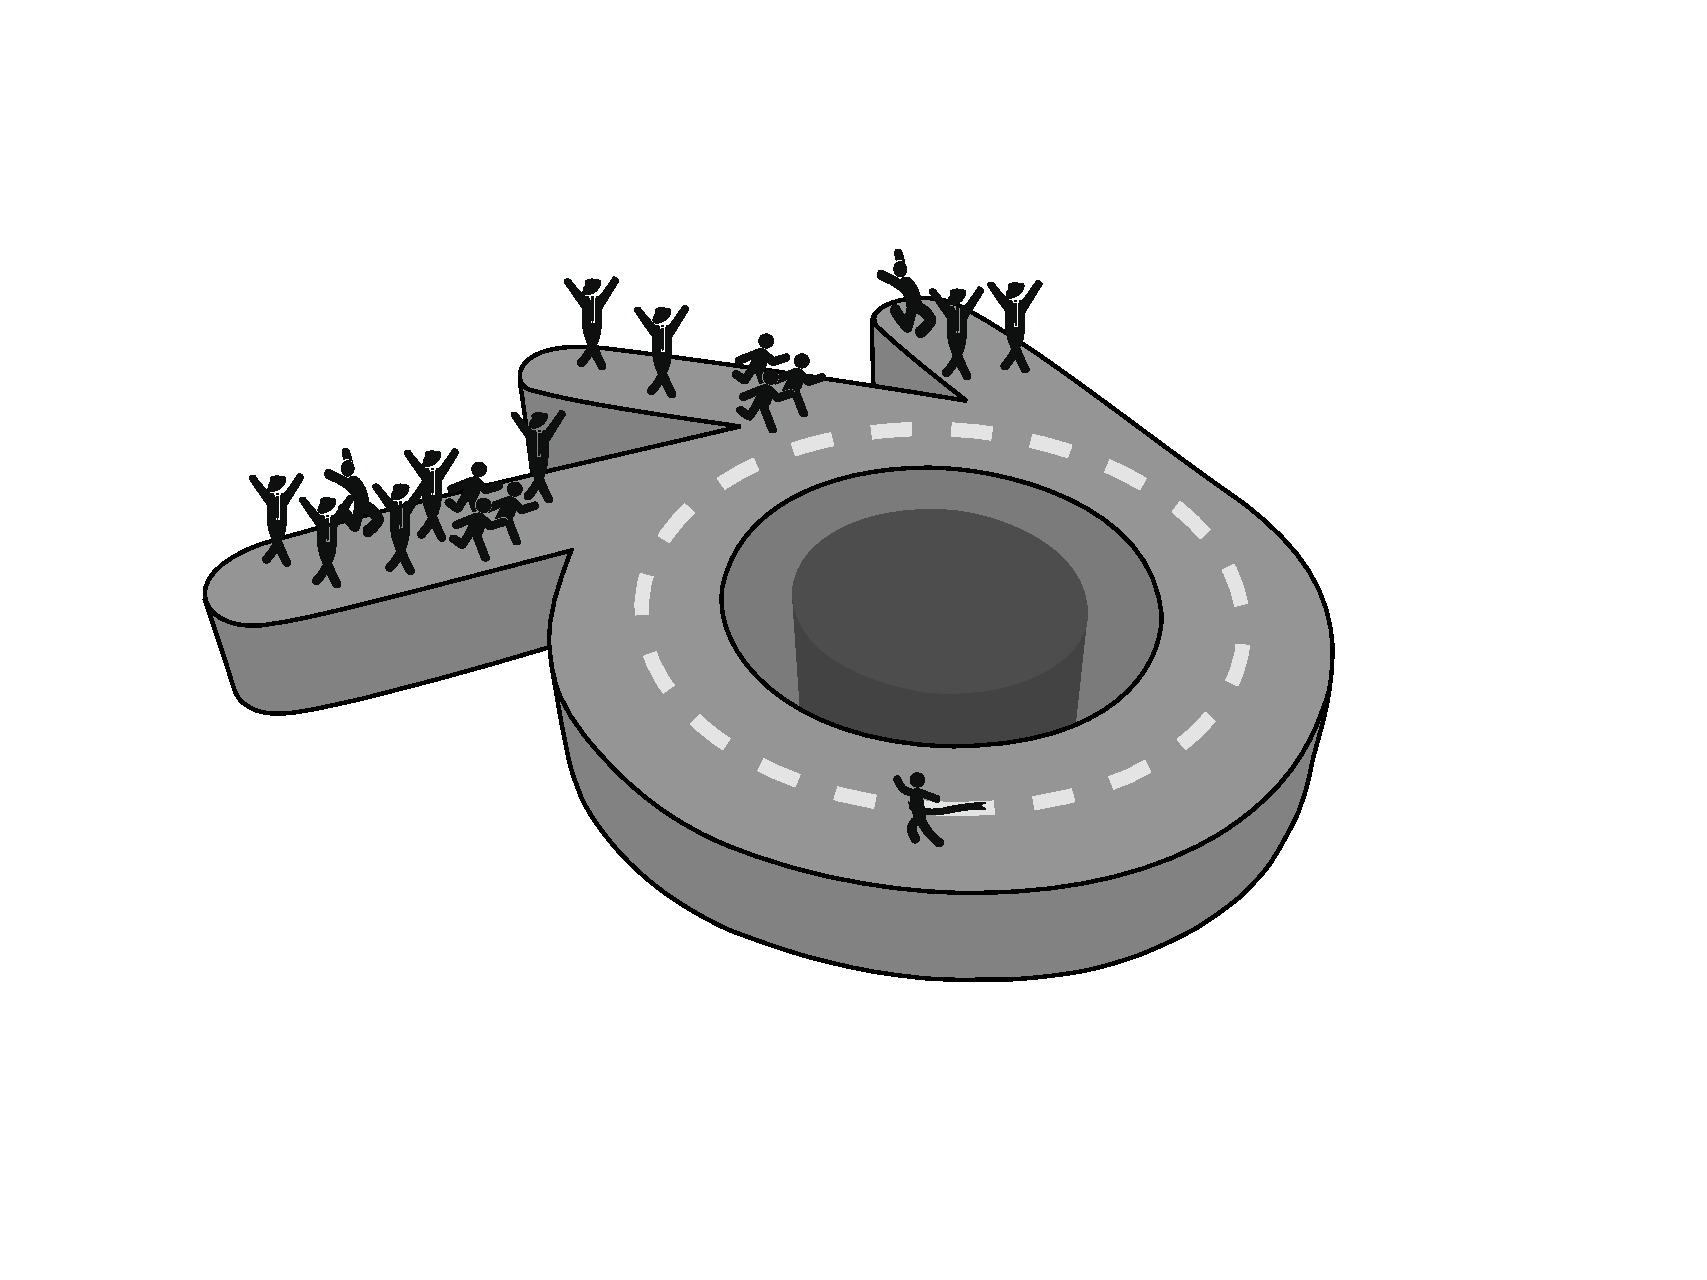
\includegraphics[width=8cm]{logo.pdf}
  \end{center}
\end{figure}
\end{frame}

\maketitle

\begin{frame}{Outline}
  \setbeamertemplate{section in toc}[sections numbered]
  \tableofcontents[hideallsubsections]
\end{frame}

\bgroup
\setbeamercolor{background canvas}{bg=black}
\begin{frame}[plain]{}
\end{frame}
\egroup

\section{What is Blend'it ?}
\begin{frame}{What is Blend'it ?}
  Blend'it is a \textbf{Blender plug-in} for \textbf{crowd animation} and \textbf{environment generation}.
  
  + screenshot
\end{frame}

\begin{frame}{A Lot of Powerful Software}


\begin{figure}
  \includegraphics<1>[width=.95\textwidth]{golaem.jpg}
  \includegraphics<2>[width=.95\textwidth]{massive.jpg}
  \includegraphics<3>[width=.95\textwidth]{VUE.jpg}
  \caption*{\only<1>{Golaem}\only<2>{Massive}\only<3>{VUE}}
\end{figure}

\end{frame}

\begin{frame}{A Lot of Expensive Software}
  \begin{itemize}
    \item Maya3D: \$1470/year
    \item Golaem: \$5000/year
    \item Massive: \$3,500 - \$16,000/year
    \item VUE: \$1700
    \item Terragen: \$600
  \end{itemize}
\end{frame}

\begin{frame}{Why Blender ?}
  Complete open-source 3D software: modelisation, animation, render, ...
    \begin{figure}
        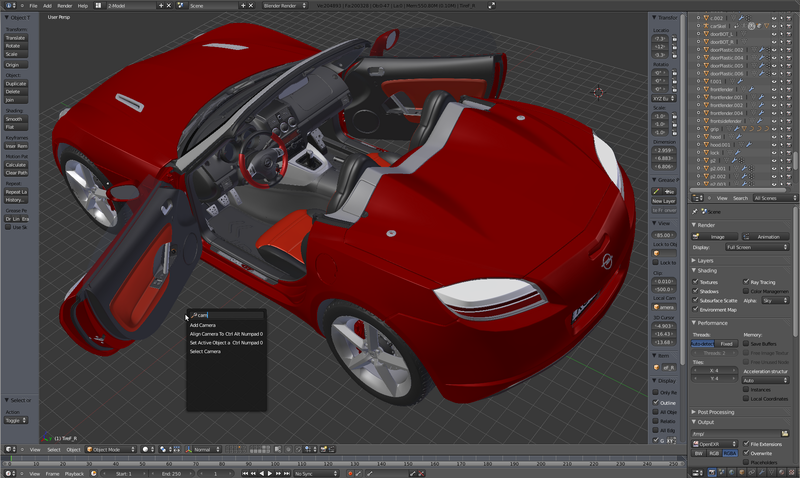
\includegraphics[width=10cm]{blender_mod}
    \end{figure}
\end{frame}

\begin{frame}{Why Blender ?}
  Powerful python API (no need to modify the source code of blender)
  \begin{figure}
        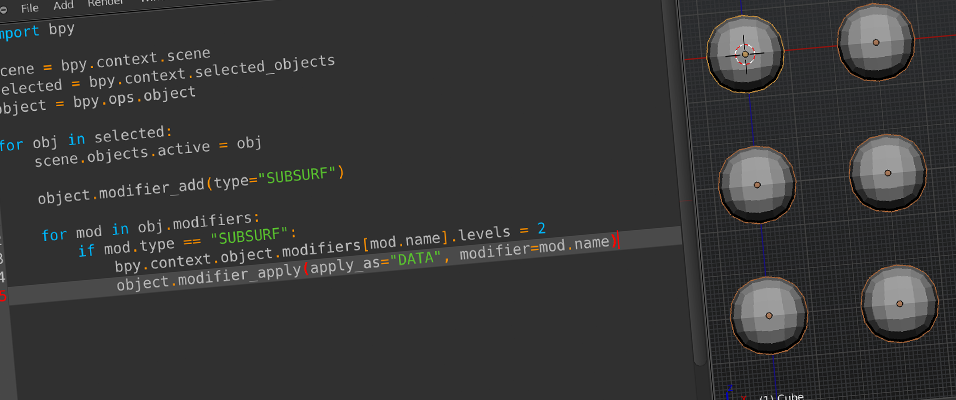
\includegraphics[width=11cm]{blender_script}
    \end{figure}
\end{frame}

\begin{frame}{Project organization}
  \begin{figure}
    \begin{center}
      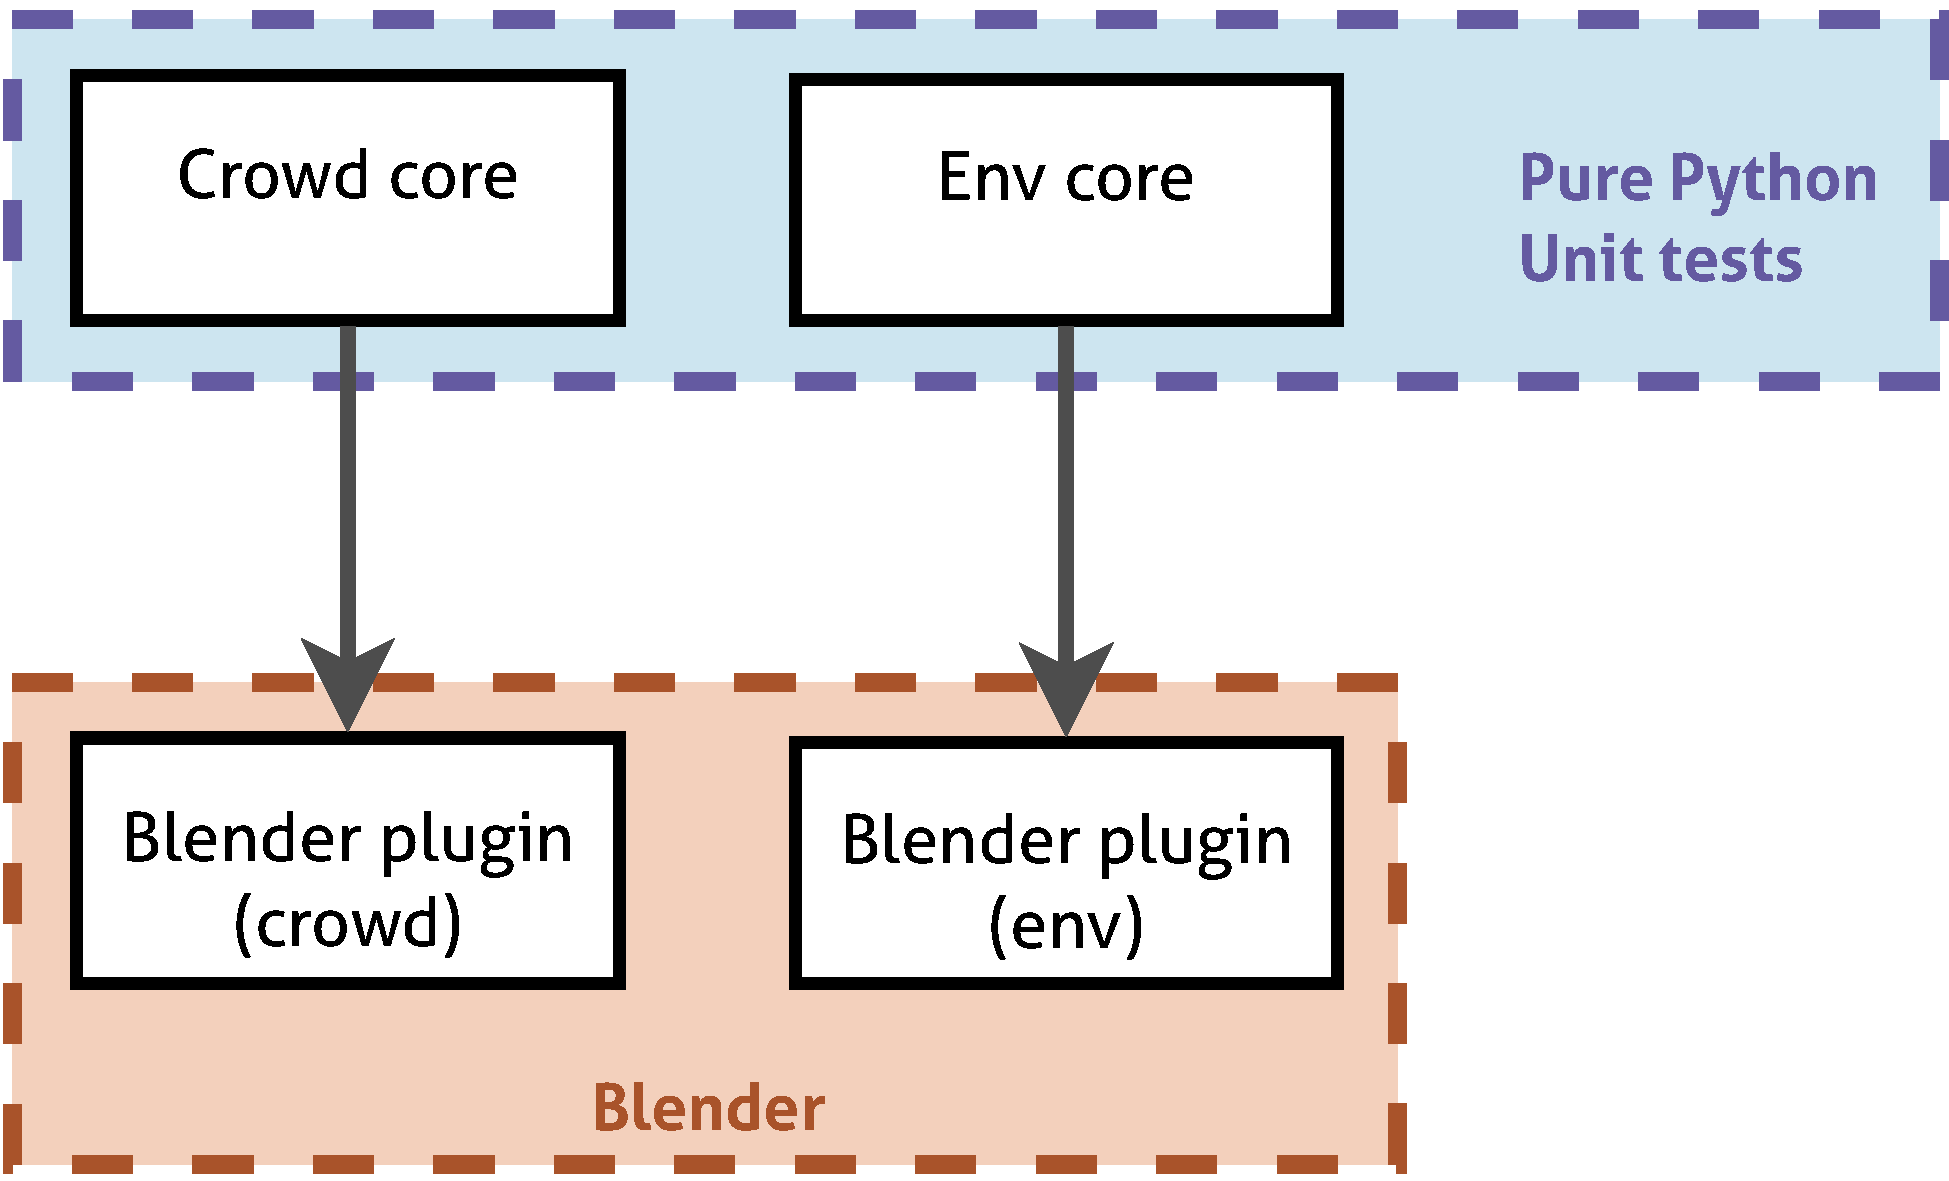
\includegraphics[width=9cm]{orga.pdf}
    \end{center}
  \end{figure}
\end{frame}


\section{Crowd Animation}
\begin{frame}{Crowd Animation - Algorithm}
  bla
\end{frame}

\begin{frame}{Demo}
\end{frame}

\begin{frame}{What is missing}
\end{frame}

\section{Environment generation}
\begin{frame}{Environment Generation - General Layout}
  \begin{figure}
    \begin{center}
      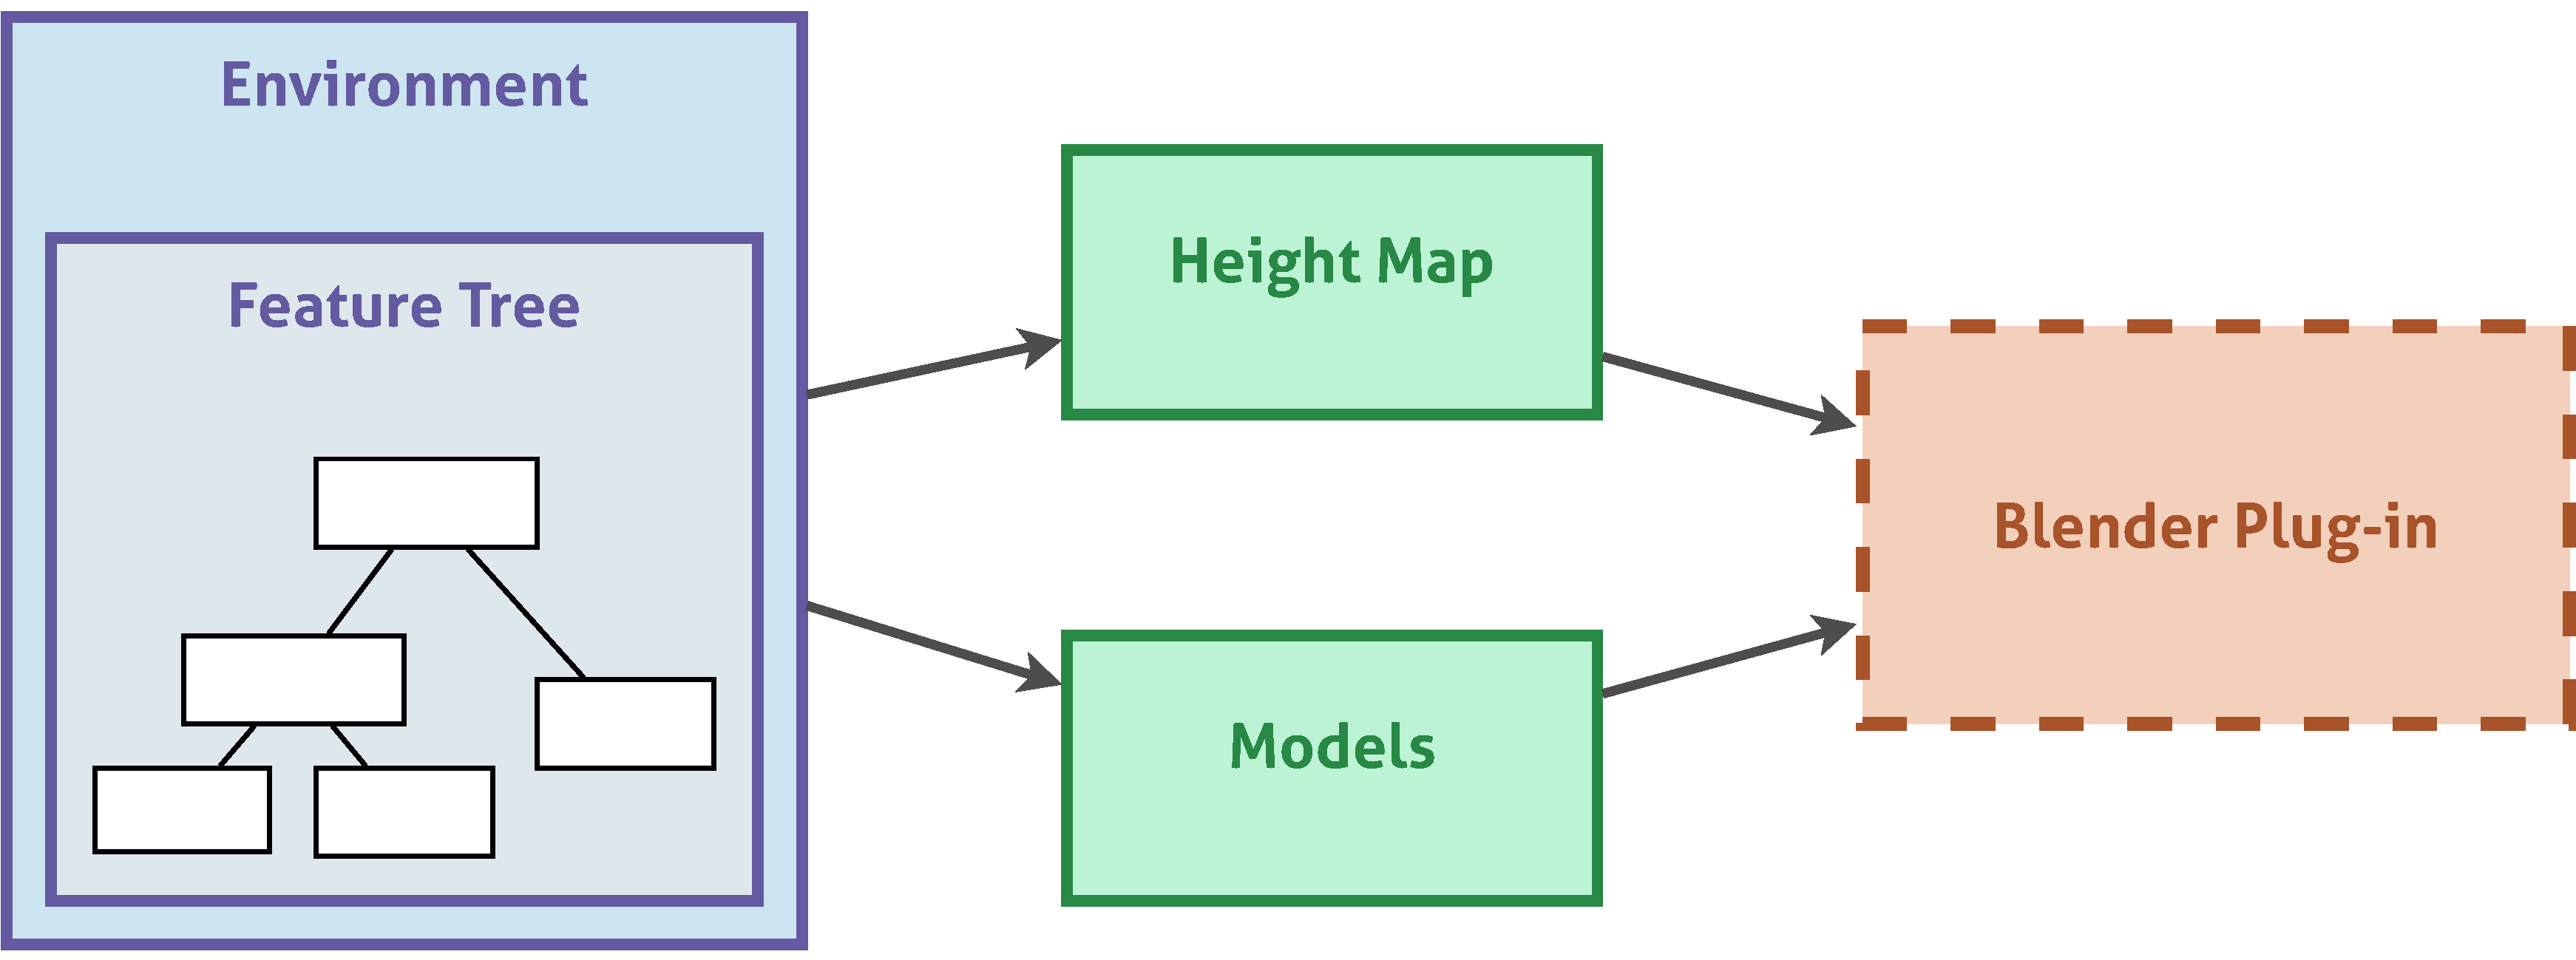
\includegraphics[width=10cm]{env_global.pdf}
    \end{center}
  \end{figure}
\end{frame}

\begin{frame}{Features}
  \begin{figure}
    \begin{center}
      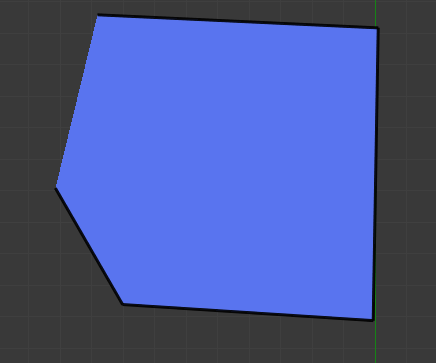
\includegraphics[width=4cm]{feature}
    \end{center}
  \end{figure}
  Feature:
  \begin{itemize}
    \item 
    \item \texttt{z(x,y)} : height function
    \item \texttt{models} : list of models
  \end{itemize}
\end{frame}

\begin{frame}{Tree Construction}
  bla
\end{frame}

\begin{frame}{Height Map Generation}
  bla
\end{frame}

\begin{frame}{Demo}
\end{frame}

\begin{frame}{What is missing}
  \begin{itemize}
    \item Live modifications
  \end{itemize}
\end{frame}

\bgroup
\setbeamercolor{background canvas}{bg=black}
\begin{frame}[plain]{}
\end{frame}
\egroup


\begin{frame}{Bibliography}
  
\end{frame}

\begin{frame}{Theme}
  Used the theme \emph{mtheme} by Matthias Vogelgesang, licensed under a Creative Commons
  Attribution-ShareAlike 4.0 International License.
\end{frame}

\end{document}
